\section{Xwindow インターフェース}
\markright{\arabic{section}. Xwindow}
Euslisp上のXwindowインターフェースは、{\tt 'eusx'}という
名前でEuslispが呼び出されたとき、実行可能となる。
\footnote{eusxは、eusへのシンボリックリンクである。}
eusxは、起動時に環境変数"DISPLAY"を参照してXserverに接続を試みるため、
自分のXseverに環境変数"DISPLAY"が正しく設定されていなければならない。

Euslispには、次の3つのレベルのXwindowインターフェースが定義されている。
(1) Xlib関数, (2) Xlibクラスと(3) XToolKitクラスである。
この節と次のXToolKitの節に記述されている
全てのXwindow関数は、"X"パッケージの中に含まれている。
それらの関数名は、元のXlib関数名から最初の"X"を省いき、全ての文字を大文字に
変更したものとなっている。
例えば{\tt XdefaultGC}は{\tt X:DEFAULTGC}と名付けられていて、
{\tt X:XDEFAULTGC}ではない。

Xlib関数は、Xwindowシステムへの低レベルインターフェースで、
foreign関数として定義されている。
これらのXlib関数は、パラメータの型チェックあるいは
パラメータの数のチェックを実行していないため、
十分注意して使用しなければならない。
例えば、すべてのXlibの呼び出しにおいてXserverとの接続を確認するために
{\tt x:*display*}を引き数として要求する。もし、指定し忘れたならば、Xlibは
エラーを通知し、そのプロセスは死ぬ。
このような不便を避け、オブジェクト指向のインターフェースを作るために、
2番めのレベルのインターフェースであるXlibクラスが備わっている。
%By instantiating the xwindow class, you will get a window on a screen,
%and sending messages to the instance, you can draw lines, strings, or whatever
%in it.
この節では、この2番めのレベルのインターフェースに焦点を当てる。
XToolKitと呼ばれるもっと高レベルのXwindowライブラリは、次節で
説明されている。

この節に記述されているクラスは、以下の継承の階層を持っている。

\begin{quote}
\begin{verbatim}
propertied-object
   viewsurface
      x:xobject
         x:gcontext
         x:xdrawable
             x:xpixmap
             x:xwindow
   colormap
\end{verbatim}
\end{quote}

\subsection{\label{xvariables}Xlibのグローバル変数とその他関数}
\begin{refdesc}
\vardesc{x:*display*}{Xのdisplay ID(整数)}
\vardesc{x:*root*}{デフォルトのroot windowオブジェクト}
\vardesc{x:*screen*}{デフォルトのscreen ID(整数)}
\vardesc{x:*visual*}{デフォルトのvisual ID(整数)}
\vardesc{x:*blackpixel*}{黒色のpixel値 = 1}
\vardesc{x:*whitepixel*}{白色のpixel値 = 0}
\vardesc{x:*fg-pixel*}{window作成時に参照されるデフォルトの文字色のpixel値、ふつう{\tt *blackpixel*}。}
\vardesc{x:*bg-pixel*}{window作成時に参照される背景色のpixel値、ふつう{\tt *whitepixel}。}
\vardesc{x:*color-map*}{システムのデフォルトカラーマップ}
\vardesc{x:*defaultGC*}{pixmap生成時に参照されるデフォルトgcontext}
\vardesc{x:*whitegc*}{文字色が白色のgcontext}
\vardesc{x:*blackgc*}{文字色が黒色のgcontext}
% \vardesc{*gray-gc*}{ハーフトーンのGC}
\vardesc{*gray-pixmap*}{{\tt (make-gray-pixmap 0.5)}の結果。}
\vardesc{*gray25-pixmap*}{
1/4のピクセルが{\tt *fg-pixel*}であり、3/4が{\tt *bg-pixel*}である16x16のpixmap。}
\vardesc{*gray50-pixmap*}{1/2のピクセルが{\tt *fg-pixel*}である16x16のpixmap。}
\vardesc{*gray75-pixmap*}{3/4のピクセルが黒色である16x16のpixmap。}
\vardesc{*gray25-gc*}{{\tt *gray25-pixmap*}から作る25\%のグレーGC。}
\vardesc{*gray50-gc*}{{\tt *gray50-pixmap*}から作る50\%のグレーGC。}
\vardesc{*gray75-gc*}{{\tt *gray75-pixmap*}から作る75\%のグレーGC。}
\vardesc{*gray*}{{\tt "\#b0b0b0"}}
\vardesc{*bisque1*}{{\tt "\#ffe4c4"}}
\vardesc{*bisque2*}{{\tt "\#eed5b7"}}
\vardesc{*bisque3*}{{\tt "\#cdb79e"}}
\vardesc{*lightblue2*}{{\tt "\#b2dfee"}}
\vardesc{*lightpink1*}{{\tt "\#ffaeb9"}}
\vardesc{*maroon*}{{\tt "\#b03060"}}
\vardesc{*max-intensity*}{65535}
\vardesc{font-cour8}{{\tt (font-id "*-courier-medium-r-*-8-*")}}
\vardesc{font-cour10}{{\tt (font-id "*-courier-medium-r-*-10-*")}}
\vardesc{font-cour12}{{\tt (font-id "*-courier-medium-r-*-12-*")}}
\vardesc{font-cour14}{{\tt (font-id "*-courier-medium-r-*-14-*")}}
\vardesc{font-cour18}{{\tt (font-id "*-courier-medium-r-*-18-*")}}
\vardesc{font-courb12}{{\tt (font-id "*-courier-bold-r-*-12-*")}}
\vardesc{font-courb14}{{\tt (font-id "*-courier-bold-r-*-14-*")}}
\vardesc{font-courb18}{{\tt (font-id "*-courier-bold-r-*-18-*")}}
\vardesc{font-helvetica-12}{{\tt (font-id "*-Helvetica-Medium-R-Normal-*-12-*")}}
\vardesc{font-lucidasans-bold-12}{{\tt (font-id "lucidasans-bold-12")}}
\vardesc{font-lucidasans-bold-14}{{\tt (font-id "lucidasans-bold-14")}}
\vardesc{font-helvetica-bold-12}{{\tt (font-id "*-Helvetica-Bold-R-Normal-*-12-"
)}}
\vardesc{font-a14}{{\tt (font-id "*-fixed-medium-r-normal-*-14-*")}}

%\vardesc{x:*reversevideo*}{}
\vardesc{x:*xwindows*}{Euslispによる子windowを含んだ全てのwindowのリストを
保持する。}
\vardesc{x:*xwindow-hash-tab*}{drawable IDからxwindowオブジェクトを
探すためのハッシュテーブル。
{\tt x:nextevent}で得られるイベント構造はwindow IDであるため、
{\tt x:window-main-loop}はこのテーブルを使用して一致するxwindowオブジェクト
を知るために{\tt x:event-window}を呼び出す。}
%\vardesc{x:gcval}{}

\funcdesc{xflush}{}{
Xlibのコマンドバッファに保有するコマンドをすべてXserverに送る。
XlibバッファがXserverに出力するため、
Xserverに発行されたコマンドは、すぐに実行されない。
これは、ネットワークの渋滞およびプロセスの切替え頻度を減少させるために
必要である。
コマンドの効果を見るためにコマンドバッファを掃き出す方法として、
{\bf xflush}を使用するかあるいは{\bf :flush}メッセージをxwindowオブジェクトに
送る。}

\end{refdesc}

\subsection{Xwindow}

\begin{refdesc}

\classdesc{Xobject}{geometry:viewsurface}{}{
すべてのXwindowに関連するクラスの共通のスーパークラスである。
現在、スロットもメソッドも定義されていない。}

\classdesc{Xdrawable}{Xobject}
{(drawable  \hspace{10mm} \=  ; drawable  ID \\
 \> gcon \>  ; this drawable's default graphic context object\\
\> bg-color \> ; background color \\
\> width height \> ; horizontal and vertical dimensions in dots}
{{\bf Xdrawable}は、線分や文字列のようなグラフィックオブジェクト
を描くための四角領域を定義する。
{\bf Xdrawable}は、xwindowやxpixmapのための共通メソッド
を定義するための抽象クラスであり、
このクラスのインスタンスは何の効果も持っていない。}

\methoddesc{:init}{id}{
{\em id}は、このdrawableのIDとして{\tt drawable}スロットに設定される。
新しいGC(graphic context)が生成され、このdrawableオブジェクトの
デフォルトGCとして{\tt gcon}に設定される。}
\methoddesc{:drawable}{}{drawable IDを返す。}
\methoddesc{:flush}{}{Xlibのバッファに保有されるコマンドを掃き出す。}
\methoddesc{:geometry}{}{
7つの幾何学属性のリストを返す。
そのリストは、root-window-id, x座標, y座標,
幅, 高さ, 枠線の幅, visualの深さである。}

\methoddesc{:height}{}{
この{\bf Xdrawable}の高さ(y軸方向のドット数)を返す。}
\methoddesc{:width}{}{
この{\bf Xdrawable}の幅(x軸方向のドット数)を返す。}
\methoddesc{:gc}{\&rest newgc}{
もし、{\em newgc}が与えられない場合、現在のGCオブジェクトを返す。
もし、{\em newgc}が{\bf gcontext}のインスタンスなら、
この{\bf Xdrawable}の{\tt gc}に設定する。
そうでなければ、{\em newgc}はメッセージとみなされ、
現在の{\tt gc}に送られる。}
\methoddesc{:pos}{}{
この{\bf Xdrawable}の位置を示す整数ベクトルを返す。
位置は親windowの相対位置としていつも定義され、
windowマネージャの仲介のもとにルートwindowの直接の子windowとして
生成されたwindowは、ルートwindowの本当の位置に関わらず、環境の
タイトルwindowの固定座標を返す。}
\methoddesc{:x}{}{この{\bf Xdrawable}の親windowとの相対的な現在のx座標を返す。}
\methoddesc{:y}{}{この{\bf Xdrawable}の親windowとの相対的な現在のy座標を返す。}
\methoddesc{:copy-from}{drw}{
{\em drw}は、他の{\bf drawable}オブジェクト(Xwindowまたはpixmap)である。
{\em drw}の内容がこの{\bf Xdrawable}にコピーされる。}

\begin{figure}
\begin{center}
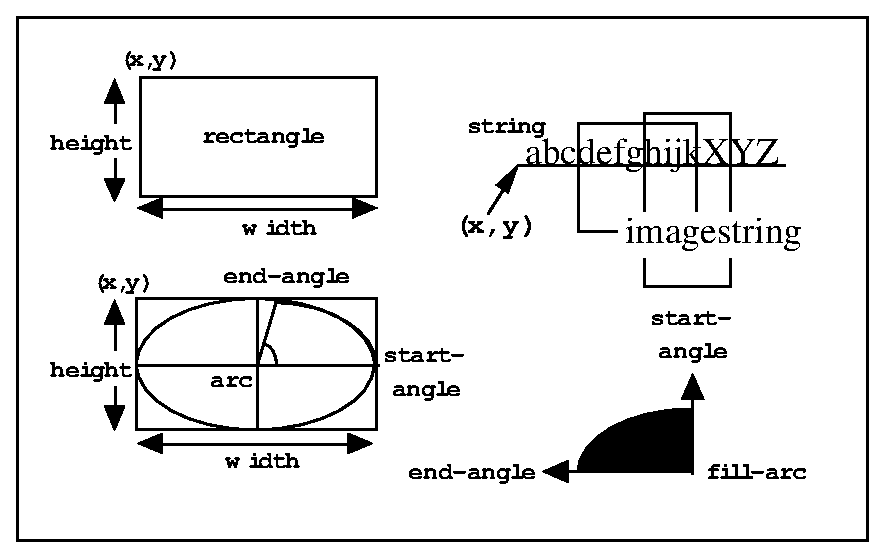
\includegraphics[height=6cm]{fig/xdraw.ps}
%\epsfile{file=fig/xdraw.ps,height=6cm}
\end{center}
\caption{描画の基本\label{xdraw}}
\end{figure}


\methoddesc{:point}{x y \&optional (gc gccon)}{
$(x, y)$の位置にオプションの{\em gc}で点を描く。}
\methoddesc{:line}{x1 y1 x2 y2 \&optional (gc gcon)}{
{\em (x1,y1)}から{\em (x2,y2)}へオプションの{\em gc}を用いて
線分を描く。{\em x1, y1, x2, y2}は整数でなければならない。}
\methoddesc{:rectangle}{x y width height \&optional (gc gcon)}{
{\em (x,y)}を中心として{\em width}の幅と{\em height}の高さを持つ
四角形を描く。}
\methoddesc{:arc}{x y width height angle1 angle2 \&optional (gc gcon)}{
{\em (x,y)}を中心として{\em width}の幅と{\em height}の高さを持つ
四角形に内接する楕円の円弧を描く。{\em angle1}が始まりの角度を示し、
{\em angle2}が終わりの角度を示す。これらの角度の単位はラジアンである。}
\methoddesc{:fill-rectangle}{x y width height \&optional (gc gcon)}{
四角領域を埋める。}
\methoddesc{:fill-arc}{x y width height angle1 angle2 \&optional (gc gcon)}{
円弧の中を埋める。}
\methoddesc{:string}{x y str \&optional (gc gcon)}{
{\em (x,y)}の位置から文字列{\em str}を表示する。背景は、書かない。}
\methoddesc{:image-string}{x y str \&optional (gc gcon)}{
文字列{\em str}を表示する。文字列は、背景色で満たされる。}
\methoddesc{:getimage}{\&key :x :y :width :height (:mask \#ffffffff) (:format 2)}{
serverからximageを取り、ピクセルデータを文字列として返す。
serverから送られるピクセルデータは、一端 Xlibのximage構造に蓄積される。
その後、行毎に文字列にコピーされる。
ximage構造は、自動的に破壊される。
{\tt :getimage}により得られた画像文字列は、{\tt pixel-image}を作るために
使用できる。また、\ref{PBMfile}節に書かれているようにpbmフォーマットのファイルに
書き込むことができる。}
\methoddesc{:putimage}{image \&key :src-x :src-y :dst-x :dst-y :width :height ((:gc g) gc)}{
この{\bf Xdrawable}の指定された位置に{\em image}を表示する。
{\em image}は、文字列あるいはximage構造へのアドレスポインターである。}
\methoddesc{:draw-line}{from to}{
{\bf :line}メソッドと同じである。
他の{\bf viewsurface}クラスとの互換性を提供できる。}
\methoddesc{:line-width}{\&optional dots}{
この{\bf Xdrawable}のデフォルトGCの線の幅を設定する。
{\tt :gc :line-width}メッセージの使用を推薦する。}
\methoddesc{:line-style}{\&optional dash}{
この{\bf Xdrawable}のデフォルトGCの線スタイルを設定する。
{\tt :gc :line-style}の使用が好まれる。}
\methoddesc{:color}{\&optional c}{この{\bf Xdrawable}の色を設定する。}
%\methoddesc{:set-show-mode}{}{
%コピーモードを設定する。この関数は、ふつう白黒ディスプレイで使用される。}
%\methoddesc{:set-erase-mode}{}{
%消去モードを設定する。この関数は、ふつう白黒ディスプレイで使用される。}
%\methoddesc{:set-xor-mode}{}{
%反転モードを設定する。この関数は、ふつう白黒ディスプレイで使用される。}
\methoddesc{:clear}{}{
全画面を消去する。この関数は、{\tt :clear-area}を呼び出す。}
\methoddesc{:clear-area}{\&key :x  :y :width :height :gc}{
{\bf :fill-rectangle}メソッドを用いて四角領域を消去する。}

\classdesc{Xpixmap}{Xdrawable}{}{
pixmapは、画像バッファあるいは背景のパターンとしてしばしば用いられる
drawableである。xwindowと異なり、xwindowにコピーされるまで
pixmap自身を見ることはできないし、pixmapはどんなイベントも発生しない。}

\methoddesc{:init}{id}{このpixmapを初期化する。}
\methoddesc{:create}{\&key (:width 500) (:height 500) (:depth 1) (:gc *defaultgc*)}{
デフォルトGCとして{\em :gc}を持つ、{\em width}$\times${\em height}のpixmapを作成する。}
\methoddesc{:create-from-bitmap-file}{fname}{
{\em file}で指定されるbitmapファイルからpixmapを作る。}
\methoddesc{:write-to-bitmap-file}{fname}{
このpixmapの内容を{\em fname}で指定されるbitmapファイルに書き込む。
このファイルは、{\bf :create-from-bitmap-file}メソッドで
pixmapを作り、読み戻すことができる。}
\methoddesc{:destroy}{}{
このpixmapを破壊し、X resourceを開放する。}

\classdesc{Xwindow}{Xdrawable}{(parent subwindows backing-store)}{
{\bf Xwindow}は、画面の見える四角領域を定義する。
これは、{\bf text-window}やグラフィックオブジェクトを描くための{\bf canvas}
だけでなく、windowというよりはむしろグラフィックオブジェクトのような
たくさんの{\bf panel-item}や{\bf scroll-bars}からも継承される。}

\longdescription{:create}{\&key ( \= (:parent *root*) \` [メソッド] \\
%\longdescription{:create}{\&key ( \= (:parent par) \hspace{98mm} [メソッド] \\
\> (:x 0) (:y 0) (:size 256) (:width size) (:height size) (:border-width 2) \\
\> (:save-under nil) (:backing-store :always) (:backing-pixmap nil)\\
\> (:border *fg-pixel*) (:background *bg-pixel*) \\
\> (:map T) (:gravity :northwest) \\
\> (:title "WINDOW") (:name title) \\
\> (:font) \\
\> :event-mask (:key :button :enterLeave :configure :motion)}
{xwindow生成し、初期化する。
{\em :parent}が与えられたとき、このwindowは{\em :parent}の子windowとして
生成され、{\em :parent}の{\tt subwindows}リストに蓄積される。
{\em :x, :y, :size, :width, :height}と{\em :border-width}は、このwindow
の位置と寸法を決定する。
{\em :save-under}と{\em :backing-store}は、windowが再マップされたときに
生じるXserverの行動を制御する。
{\em :backing-store}は{\tt :notUseful, :WhenMapped, :Always}のどれかであるが、
{\em :save-under}はTあるいはNILである。
{\em :backing-pixmap}がTのとき、このwindowと同じサイズのpixmapがEuslispにより
生成され、もしXserverが{\tt backing-store}の容量を持っていない場合は、
backing-storeとして蓄積される。
{\em :border}と{\em :background}は、{\tt border\_pixel}と
{\tt background\_pixel}属性をそれぞれ指定する。
もし、{\bf panel}の中のpanel-buttonとしてたくさんの小さなwindowを
作成するような場合で、このwindowが生成後にすぐ表示されるべきでないならば、
{\em :map}はNILにセットされなければならない。
{\em :title}は、windowのタイトルバーに現れるwindowのタイトルである。
{\em :name}は、このwindowのplistに蓄積されるwindowの名前であり、
プリンタにより表示される名前である。
このwindowへのXのイベントは、{\em :event-mask}によって決定される。
それはビットで構成されるevent-maskの整数表現あるいは次のsymbolのリスト
である。
{\tt :key, :button, :enterLeave, :motion}と{\tt :configure}。
もし、もっと正確な制御が必要ならば、次のsymbolをそれぞれのイベントに
指定することができる。{\tt :keyPress, :keyRelease, :ButtonPress, :ButtonRelease,} 
{\tt :EnterWindow, :LeaveWindow, :PointerMotion, :PointerMotionHint,} 
{\tt :ButtonMotion, :KeyMapState,\\ :Exposure, :VisibilityChange,}
 {\tt :StructureNotify,
:ResezeRedirect, :SubstructureNotify,\\ :SubstructureRedirect,} {\tt
:FocusChange, :PropertyChange, :ColormapChange}と\\{\tt :OwnerGrabButton}。
{\tt :key}は、{\tt :keyPress}と{\tt :KeyRelease}の両方が指定でき、
{\tt :button}は、{\tt :ButtonPress}と{\tt :ButtonRelease}の両方が指定できる。
サーバからイベントが送られてきたとき、{\bf window-main-loop}は、
そのイベント構造を解析し、{\tt :KeyPress, :KeyRelease, :buttonPress,} {\tt
:ButtonRelease, :EnterNotify,} {\tt :LeaveNotify, :MotionNotify, :ConfigureNotify}
メッセージをそのイベントが発生したwindowに送る。}

\methoddesc{:map}{}{この{\bf Xwindow}とその子windowを全て表示する。}
\methoddesc{:unmap}{}{この{\bf Xwindow}をとその子windowを全て非表示にする。}
\methoddesc{:selectinput}{event-mask}{
{\em event-mask}は、整数かあるいはイベントマスクsymbolのリストである。
ビットが1となっているかあるいは{\em event-mask}リスト
に列挙されているイベントは、それぞれこのwindowに通知される。}
\methoddesc{:destroy}{}{この{\bf Xwindow}を破壊し、X resourceを開放する。
windowオブジェクトは、ガーベージコレクトされないため、
{\tt *xwindow*}や{\tt *xwindow-hash-tab*}の中の一致するエントリも削除される。
全ての子windowも{\tt :destroy}を送ることにより削除する。
このwindowは、親windowの子windowのリストから削除される。
{\tt drawable}IDは、NILに設定される。}
\methoddesc{:parent}{}{親windowオブジェクトを返す。}
\methoddesc{:subwindows}{}{
全ての子windowのリストを返す。
子windowは、もっとも最近作られたものがリストの最初である。
このwindowの直接の子windowだけがリストされ、子windowの子windowは
リストされない。}
\methoddesc{:associate}{child}{
このwindowの子windowとして{\em child} windowを登録する。}
\methoddesc{:dissociate}{child}{
子windowのリストから{\em child} windowを削除する。}

%\methoddesc{:save}{}{
%copies the content of this window to the backing-store pixmap.}

%\methoddesc{:refresh}{}{
%copies from the backing-store.}

\methoddesc{:title}{title}{
このwindowのタイトル名を変更する。そのタイトル名はXserverに送られるため、
一旦蓄積され、window managerによって表示される。}

\methoddesc{:attributes}{}{このwindowの属性を表現する整数ベクトルを返す。}
\methoddesc{:visual}{}{この{\bf Xwindow}のvisual resource IDを返す。}
\methoddesc{:screen}{}{この{\bf Xwindow}のscreen resource IDを返す。}
\methoddesc{:root}{}{root window IDを返す。} 

\methoddesc{:location}{}{
このwindowのxとy座標を記述する2次元の整数ベクトルを返す。}
\methoddesc{:depth}{}{
このwindowの深さ(カラープレーンの数)を返す。}
\methoddesc{:size}{}{このwindowのサイズ(高さと幅)を返す。}
\methoddesc{:colormap}{}{このwindowのcolormap resource IDを返す。}
\methoddesc{:move}{newx newy}{
このwindowの位置を{\em (newx,newy)}に変更する。
位置は、親windowの相対位置で与えられる。}
\methoddesc{:resize}{width height}{
このwindowのサイズを変更する。
たぶん、大きさのパラメータがクライアント側のXlibに中にキャッシュされるため、
{\bf :resize}の直後に{\tt :geometry}メッセージを
送ると誤った(古い)結果を返す。}
\methoddesc{:raise}{}{このwindowを前面に持ってくる。}
\methoddesc{:lower}{}{このwindowを後ろに置く。}
\methoddesc{:background}{pixel}{
背景のピクセル値(カラーマップのインデックス)を{\em pixel}に変更する。
{\em pixel}値は、{\tt bg-color}スロットにも保存される。
{\tt :clear}処理は、現在の背景を指定された{\em pixel}で埋める。}

\methoddesc{:background-pixmap}{pixmap}{
背景のpixmap値を{\em pixmap}に変更する。}
\methoddesc{:border}{pixel}{
このwindowの枠線の色を{\em pixel}に設定する。}
%\methoddesc{:line-style}{style}{sets style attribute of GC.}
%\methoddesc{:line-width}{width}{sets width attribute of GC.}
%\methoddesc{:write-to-bitmap-file}{fname}{
%dumps the content of the backing-store pixmap to a bitmap-file.}
%\methoddesc{:draw-line}{from to}{
%a line is drawn in both this window and the backing-store.}
\methoddesc{:set-colormap}{cmap}{colormapを設定する。}
\methoddesc{:clear}{}{
この{\bf Xwindow}内を全て消去する。}
\methoddesc{:clear-area}{\&key :x :y :width :height}{
この{\bf Xwindow}の指定された四角領域を消去する。}
%\methoddesc{:who-is-parent}{\&optional obj}{
%{\em obj}の親windowを返す。もし、{\em obj}がなければ、この{\bf Xwindow}の
%親windowを返す。}

\funcdesc{make-xwindow}{\&rest args}{
引き数{\em args}で示される{\bf Xwindow}を作る。}
\funcdesc{init-xwindow}{\&optional (display (getenv "DISPLAY"))}{
eusxが起動するときに最初に呼び出される関数である。
{\bf init-xwindow}は、{\em display}で指定されるXserverに接続し、
\ref{xvariables}節に記述されているデフォルト変数を初期化する。
{\bf init-xwindow}は、デフォルトフォントをロードし、
グローバル変数に設定する。例えば、font-courb12, lucidasans-bold-12など。
このフォントロードは、起動時に時間遅れを引き起こす。
フォントロードの数を減らしたり、ワイルドカード文字"*"を使用せずに
正確なフォント名を指定することにより、その遅れを短くできる。}

%\funcdesc{switchvideo}{}{
%文字色と背景色を交換する。
%この関数は、一般に白黒ディスプレイで使用される。}
%\funcdesc{reversevideo}{}{
%文字色に白色を設定し、背景色に黒を設定する。
%この関数は、一般に白黒ディスプレイで使用される。}

\subsection{Graphic Context}

\classdesc{gcontext}{Xobject}{(gcid GCValues)}{graphic context(GC)を定義する。
Euslispの中で、全てのwindowはデフォルトGCを持っている。}

\longdescription{:create}{\&key \= (:drawable defaultRootWindow) \` [メソッド]\\
\> (:foreground *fg-pixel*) (:background *bg-pixel*) \\
\> :function :plane-mask \\
\> :line-width :line-style :cap-style :join-style \\
\> :font :dash \\}{
与えられた属性でGCを作成する。
{\em drawable}は、画面と画面の深さを知るためにXserverにより使用される。
結果のGCは、同じ画面上で作成される限り、
どのdrawableでも使用できる。}

\methoddesc{:gc}{}{XのGC IDを返す。}
\methoddesc{:free}{}{この{\bf GC}を開放する。}

\methoddesc{:copy}{}{この{\bf GC}のコピーを作る。}
\methoddesc{:foreground}{\&optional color}{もし、{\em color}が与えられたならば、
文字色に{\em color}を設定する。{\em color}はピクセル値である。}
\methoddesc{:background}{\&optional color}{もし、{\em color}が与えられたならば、
背景色に{\em color}を設定する。{\em color}はピクセル値である。}
\methoddesc{:foreback}{fore back}{一度に文字色と背景色を設定する。}
\methoddesc{:planemask}{\&optional plane-mask}{plane-maskを設定する。}

\methoddesc{:function}{x}{描画機能を設定する。
{\em x}は、以下に示す数字かキーワードの内の1つである。
{\tt 0=Clear, 1=And, 2=AndReverse, 3=Copy, 4=AndInverted, 5=NoOp, 6=Xor, 7=Or,
8=Nor, 9=Equiv, 10=Invert,\\ 11=XorReverse, 12=CopyInverted, 13=OrInverted,
14=Nand, 15=Set, :clear, :and,\\ :andReverse, :copy, :andInverted,
:NoOp, :Xor, :Or, :Nor, :Equiv, :Invert, :XorReverse,\\ :CopyInverted,
:OrInverted, :Nand, :Set}}

\methoddesc{:font}{x}{
このGCのフォント属性を設定する。
{\em x}は、フォント名あるいはフォントIDである。
もし、{\em x}がフォント名(文字列)であったならば、{\bf :font}は
フォントIDを決めるために{\bf x:LoadQueryFont}を呼び出す。
もし、見つからなかった場合、{\tt "no such font ..."}が警告される。
もし、{\em x}がNIL(与えられなかった)ならば、このGCの現在の
フォントIDが返される。}

\methoddesc{:line-width}{x}{線幅をピクセル数{\em x}で設定する。}
\methoddesc{:line-style}{x}{線スタイル(実線、点線など)を設定する。}
\methoddesc{:dash}{\&rest x}{{\em x}のそれぞれの要素は、整数である。
{\bf :dash}は、線スタイルの点線パターンを設定する。}
%\methoddesc{:color}{c}{文字色を{\em c}に設定する。}
\methoddesc{:tile}{pixmap}{{\em pixmap}をこのGCのタイルパターンに設定する。}
\methoddesc{:stipple}{pixmap}{{\em pixmap}をこのGCの点画に設定する。}
\methoddesc{:get-attribute}{attr}{属性値を得る。
{\em attr}は、{\tt :function, :plane-mask, :foreground,
:background, :line-width, :line-style, :cap-style, :join-style,
:fill-style, :fill-rule, :font}の内の1つである。
属性値を表す整数が返される。}

\longdescription{:change-attributes}{\&key \= :function :plane-mask :foreground :background
\`[メソッド]\\
\>:line-width :line-style :cap-style :join-style :font :dash}{
属性値を変更する。
同時に複数の属性値を変更できる。}

%\funcdesc{make-color-gc}{color}{{\em color}で指定される{\bf GC}を作り、
%この{\bf GC}を返す。}

\funcdesc{font-id}{fontname}{
もし、{\em fontname}が整数であるなら、フォントIDとみなしてその値を返す。
もし、{\em fontname}が文字列であるなら、{\bf x:LoadQueryFont}を使用して
フォント構造を得て、そのフォントIDを返す。
{\em fontname}は、正確な名前の略語でも良い。例えば、
24ポイントのクーリエフォントとして{\tt "*-courier-24-*"}を指定できる。
もし、フォントが見つからなければ、{\tt can't load font}の警告を
出力する。}

\funcdesc{textdots}{str font-id}{
{\em str}文字列のascent descent widthをドット単位に示す3つの整数のリストを
返す。}

\end{refdesc}

\subsection{色とカラーマップ}

\begin{refdesc}
\classdesc{colormap}{object}
{(cmapid planes pixels LUT-list)}{
{\bf Xwindow}のカラーマップおよびアプリケーション指向のカラールックアップテーブル
を定義する。
カラーはRGB値で表現され、その範囲は0〜65535である。
カラーマップのカラーセルは、8ビットの擬似カラーディスプレイの上の
0〜255の範囲の値に設定される。}
\end{refdesc}

ここで、8ビットの擬似カラーディスプレイの機能があり、
256色を選択することができると仮定する。
基本的にカラーマップを使用する2つの方法がある。
1つは、システムデフォルトのカラーマップを共有する方法で、
もう1つはプロセスに独自のカラーマップを作成する方法である。
もし、システムのデフォルトカラーマップを使用する場合、
マップのすべてのカラーセルを使いきらないように注意しなければならない。
なぜなら、マップは多くののプロセスから共有されているからである。
もし、独自のカラーマップを使用する場合、
他のプロセスを気にすることなく256色すべてを使用することができる。
しかし、そのマップは明確に独自のwindowに設定しなければならない。
マウスのポインターがwindow内のどこかに動かされたとき、
カラーマップはwindow managerにより活性化される。

システムデフォルトのカラーマップは
eusxが実行される最初に{\bf x:colormap}のクラスのインスタンスとして、
{\bf x:*color-map*}に設定されている。
もし、独自のカラーマップを使用するとき、{\bf x:colormap}のインスタンスを
作る。
これらのインスタンスは、x serverで定義されたcolormapオブジェクトと
一致しており、それぞれのインスタンスの{\tt cmapid}に示されている。

システムデフォルトのカラーマップを使用するとき、
他のプロセスと共有するカラーを読み込み専用({\em read-only})に、
Euslispの独自カラーを読み書き可能({\em read-write})に定義することができる。
"読み込み専用"は、カラーセルに割り当てられる
任意のカラーに定義することができる。
しかし、割り当てた後変更することができない。
もう一方で、"読み書き可能"カラーは定義した後でさえ、変更することができる。
共有カラーは、他のプロセスが変更を予期していないため"読み込み専用"である。
この"読み込み専用"と"読み書き可能"の属性は、それぞれのカラーに付けられる。
(しばしば、カラーセルとして参照される)

{\bf colormap}オブジェクトは、color IDからRGBの物理的な表現への変換を
定義する。
しかしながら、これらの論理的なcolor IDは、任意に選択することができない。
特に、システムのデフォルトのカラーマップを使用しているとき、使用できない。
color ID(しばしば'pixel'として参照される)は、カラーマップの特別な色
のインデックスである。
Xlibは、割り当ての要求があると、共有カラーのために空いたインデックスの
1つを選択する。
したがって、たくさんのグレー階調のカラーを連続的に割り当てることを
保証することあるいは最初(0番目)のインデックスから始めることはできない。

アプリケーションの観点から、もっと論理的なカラー名が必要とされる。
例えば、グレー階調の数は明るさをインデックスとして参照すべきである。
レイトレーシングプログラムは、
HLSで定義される違った明るさのカラーのグループのために
連続的なインデックスの割り当てを要求する。

この問題に対処するために、Euslispのカラーマップはルックアップテーブル(LUT)
と呼ばれる別の変換テーブルを提供している。
論理的なカラーグループのために、LUTを定義でき、symbol名を付けることができる。
1つ以上のLUTをカラーマップとして定義できる。
LUTは、Xserverが認識できるように、アプリケーションが指定した論理カラーの
インデックスを物理ピクセル値に変換するために整数ベクトルである。
 
\begin{refdesc}

\methoddesc{:id}{}{{\tt cmapid}を返す。}
\methoddesc{:query}{pix}{指定されたピクセル数のRGB値を返す。}
\methoddesc{:alloc}{pix r g b}{
このメソッドは、{\tt :store nil r g b}と同一である。
新しいカラーセルがこのカラーマップに配置され、指定されたRGB値に割り当てられる。}
\methoddesc{:store}{pix r g b}{{\em pix}番目のカラーセルのRGB値を設定する。}
\methoddesc{:store}{pix color-name}{
{\bf :store}は、カラーマップに色を設定する低レベルメソッドである。
1つの書式として、RGB値を0〜65535で指定する方法である。
他の書式として、"red" や"navy-blue"のようなカラー名で指定する。
もし、{\em color-name}がなければ、NILを返す。
ピクセルはカラーマップのインデックスあるいはNILである。
もし整数なら、カラーセルは読み書き可能でなければならない。
もしNILなら、共有の読み込み専用カラーセルが割り当てられている。
{\bf :store}は、カラーマップ内のカラーセルのインデックスを返す。}

\methoddesc{:store-hls}{pix hue lightness saturation}{
HLS(Hue, Lightness and Saturation)で
指定される色をカラーマップの{\em pix}番目に蓄積する。
もし、{\em pix}がNILなら、共有の読み込み専用のカラーセルが割り当てられる。
{\bf :store-hls}は、カラーセルに割り当てられるインデックスを返す。}

\methoddesc{:destroy}{}{この{\bf colormap}を破壊し、リソースを空にする。}
\methoddesc{:pixel}{LUT-name id}{
{\em LUT}の中から{\em id}番目を調べて、ピクセル値を返す。
{\em LUT-name}は、{\tt :define-LUT}で定義されたルックアップテーブルの名前である。}

\methoddesc{:allocate-private-colors}{num}{
独自のカラーマップに{\em num}個のカラーセルを割り当てる。}

\methoddesc{:allocate-colors}{rgb-list [private]}{
{\em rgb-list}のそれぞれの要素は、red,green,blueのリストである。
カラーセルは、それぞれのRGB値が割り当てられ、ピクセル値を要素とする
整数ベクトルを返す。}

\methoddesc{:define-LUT}{LUT-name rgb-list [private]}{
{\em rgb-list}に記述されたカラーが割り当てられ、
LUTが{\em LUT-name}のシンボリック名で登録される。
独自のカラーセルを定義するためには、{\em private}をTに設定すること。}

\methoddesc{:define-gray-scale-LUT}{LUT-name levels [private]}{
線形のグレースケールカラーで表現される{\em levels}階調の
カラーセルを割り当て、LUTを返す。
例えば、{\tt (send x:*color-map* :define-gray-scale-LUT 'gray8 8)}
は、システムのデフォルトカラーマップの中に8つのグレーカラーを配置し、
{\tt \#i(29 30 31 48 49 50 51 0)}のような整数ベクトルを返す。
物理ピクセル値は、{\tt :pixel}メッセージを送ることにより得られる。
例えば、{\tt (send x:*color-map* :pixel 'gray8 2)}は、31を返す。}
 
\methoddesc{:define-rgb-LUT}{LUT-name red green blue [private]}{
RGB表現を縮小したLUTを定義する。
例えば、もし、{\em red}={\em green}={\em blue}=2なら、カラーセルには$2^{2+2+2}=2^6=64$
が割り当てられる。}
\methoddesc{:define-hls-LUT}{LUT-name count hue low-brightness
high-brightness saturation [private]}{
HLSで使用する{\em count}数のカラーを配置する。
{\em hue} (0..360),{\em saturation} (0..1),{\em low-brightness}
と{\em high-brightness}の明るさの差をカラーマップに蓄積される。
{\em LUT-name}で名付けられるLUTも作られる。}

\longdescription{:define-rainbow-LUT}{\= LUT-name count \` [メソッド]\\
\> (hue-start 0) (hue-end 360)\\
\> (brightness 0.5)\\
\> (saturation 1.0) (private nil)}{
HLSモデルを用いて{\em count}の色を配置する。
{\em brightness} (0..1)と
{\em saturation} (0..1)と,
{\em hue-start}と{\em hue-end}間の異なったhueを持つ色を
カラーマップに蓄積する。
{\em LUT-name}を名付けられたLUTも生成される。}

\methoddesc{:LUT-list}{}{このカラーマップに定義されている全てのLUTのリストを返す。
リストのそれぞれのエントリは、LUT名と整数ベクトルの組である。}
\methoddesc{:LUT-names}{}{このカラーマップの全てのLUTの名前のリストを返す。}
\methoddesc{:LUT}{name}{{\em name}で指定される整数ベクトル(LUT)を返す。}
\methoddesc{:size}{LUT}{{\em LUT}の長さを返す。}
\methoddesc{:planes}{}{このカラーマップのプレーンを返す。}
%\metdesc{:planes-bits}{}
%\metdesc{:planes-shifts}{}

\methoddesc{:set-window}{xwin}{
このカラーマップを{\em xwin}のwindowと関連付ける。
このカラーマップは、{\em xwin}にカーソルが入ったとき活性化される。}
\methoddesc{:free}{pixel | LUT}{{\em pixel}の場所にあるカラーセルを開放するか
あるいは{\em LUT}のすべてを開放する。}
\methoddesc{:init}{[cmapid]}{
このカラーマップを{\rm cmapid}で初期化する。
登録されたLUTはすべて捨てられる。}
\methoddesc{:create}{\&key (planes 0) (colors 1) (visual *visual*) (contiguous i
l)}
{新しいカラーマップを作成する。}

\classdesc{XColor}{cstruct}
{((pixel        :integer) \\
\>  (red          :short) \\
\>  (green        :short) \\
\>  (blue         :short) \\
\>  (flags        :byte) \\
\>  (pad          :byte))}{
RGBモデルのカラーを定義する。
それぞれのスロットに値を割り当てるには、{\bf setf}を用いる。
RGB値は、符合拡張され、最大値は$-1$と表現される。}

\methoddesc{:red}{}{この{\bf XColor}の赤色の値を返す。}
\methoddesc{:blue}{}{この{\bf XColor}の青色の値を返す。}
\methoddesc{:green}{}{この{\bf XColor}の緑色の値を返す。}
\methoddesc{:color}{}{この{\bf XColor}のRGB値のリストを返す。}
\methoddesc{:init}{pix R G B \&optional (f 7)}{
{\bf XColor}を初期化する。}

\funcdesc{find-visual}{type depth \&optional (screen 0)}{
{\em type}と{\em depth}で指定されるvisual-IDを見つける。
{\em type}は、{\tt :StaticGray, :GrayScale,
:StaticColor, :pseudoColor, :TrueColor}あるいは{\tt :DirectColor}のどれかである。
ふつう、{\em depth}は1, 8 または 24である。}

\end{refdesc}

\newpage

